\documentclass[12pt]{article}
\usepackage[margin=1in]{geometry}
\usepackage{amsfonts, amsmath, amssymb}
\usepackage{polynom}
\usepackage{hyperref}
\usepackage{mathtools}
\hypersetup{
    colorlinks=true,
    linkcolor=blue,
    filecolor=magenta,      
    urlcolor=cyan,
}
\usepackage{graphicx}

\usepackage{fancyhdr}
\setlength{\headheight}{15pt}
\usepackage{graphicx}


\pagestyle{fancy}
\fancyhf{}

\rhead{
  Shengdong Li
  Calc 3
}

\rfoot{
  Page \thepage
}

\usepackage{indentfirst}

\begin{document}
\title{In Conclusion}
\author{by Shengdong Li}
\date{4 October 2020}
\maketitle

\section{About the Slope Field}

Because nobody made a slope field in reply to my initial post, I decided to create one using the Desmos Slope Field Generator and make observations of that instead.

\begin{figure}[h]
  \begin{center}
    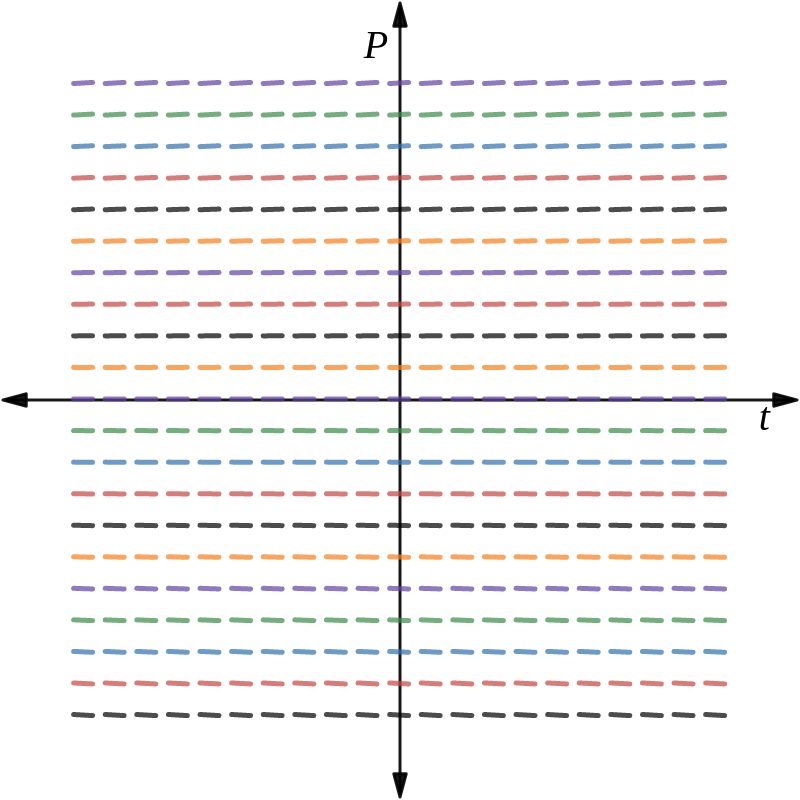
\includegraphics[scale=.3]{disc-3-conc-slope-field.png}
    \caption{\textit{Picture of slope field for $\frac{dP}{dt}=0.006P$.}}
  \end{center}
\end{figure}

One thing that I notice about this slope field is that there is a trivial, unstable equilibrium when $P=0$. This makes sense because a population cannot grow if there is none in the first place. Another thing that I noticed is that $t$ has no impact on the population growth whatsoever. This means that the rate of change of the population does not change over time, which, noting what Ankur and Daphne said in reply to my initial post, is not very realistic at all.

% texorpdfstring to get rid of href error in a title/heading for the paper. Lg is best approximation
\section{Solving for a data point}
I decided to pick the point $(2015, P)$ to solve for using my model, $P=1804.007e^{.006t}$
\begin{align}
  P         & =1804.007e^{.006\left(2015\right)} \\
  P         & =321261368.181...                  \\
  \Aboxed{P & \approx321261369}
\end{align}
\setcounter{equation}{0}

\subsection{Verifying and Analyzing Solution}
To verify my solution I decided to use \href{https://www.worldometers.info/world-population/us-population/}{Worldometer}, the same site in which I got my original data from. In the site, the recorded population for 2015 was $320,878,310$.

We can calculate the $\%error$ as follows...
\begin{align}
  \%\:error & = \frac{calculated-actual}{actual}\cdot100     \\
            & =\frac{321261369-320878310}{320878310}\cdot100 \\
            & \approx\boxed{.11\%}                           \\
\end{align}

A 0.11\% error is pretty decent margin for such a simple model in my opinion, though 2015 is very close to 2019, and farther away the accuracy definitely falls off.
\end{document}